%!TEX root = PhD_Thesis.tex
\chapter{Introduction}

%%%%%%%%%%%%%%%%%%%%%%%%%%%%%%%%%%%%%%%%%%%%%%%%%%%%%%%%%%%%%%%%%%%%%%%%%%%%%%%%%%%%%%%%%%%%%%%%%%%%======================================================================
\section{Motivation}
%======================================================================
%%%%%%%%%%%%%%%%%%%%%%%%%%%%%%%%%%%%%%%%%%%%%%%%%%%%%%%%%%%%%%%%%%%%%%%%%%%%%%%%%%%%%%%%%%%%%%%%%%%
%\subsection{Percutaneous Interventions}
%Needles are slim metal tubes with sharpened tips that puncture the skin and other intervening tissues to allow access to internal anatomy. Needles are ubiquitous tools in modern medicine. They are applied in a range of form factors by clinicians in many specialties to inject drugs, drain fluids, remove tissue samples for testing, or deposit implants. Interventional radiology is a medical specialty that uses instruments inserted through needles under medical image guidance to treat disease. Such percutaneous interventions are increasingly favored as alternatives to surgery, because they result in less trauma to the patient, and thus reduce the risk of complications and patient recovery time. 

\subsection{Liver Cancer}
The liver is a glandular organ that sits in the right side of the abdomen in humans. It weighs approximately 1.2~kg to 1.5~kg, and is approximately 14~cm long on average in adults~\cite{Wolf1990,Kratzer2003}. The liver's primary function is to filter blood coming from the digestive tract before it passes on to the rest of the body. Structurally, the liver is divided into four lobes, the left, right, caudate, and quadrate lobes. Fig.~\ref{fig:Ch1LiverAnatomy} shows the left and right lobes, which are the largest. The liver is made up of very soft tissues called parenchyma, surrounded and supported by a tough capsule. The liver receives nutrient-rich, oxygen-poor blood from the spleen, pancreas and intestines through the hepatic portal vein. The liver also receives oxygen-rich blood through the hepatic artery. Blood from the two supplies mixes as it passes through the liver lobules, the basic functional units of the liver parenchyma. Blood then passes through the hepatic veins to the inferior vena cava, through which it returns to the heart.

\begin{figure}[!ht]
\centering
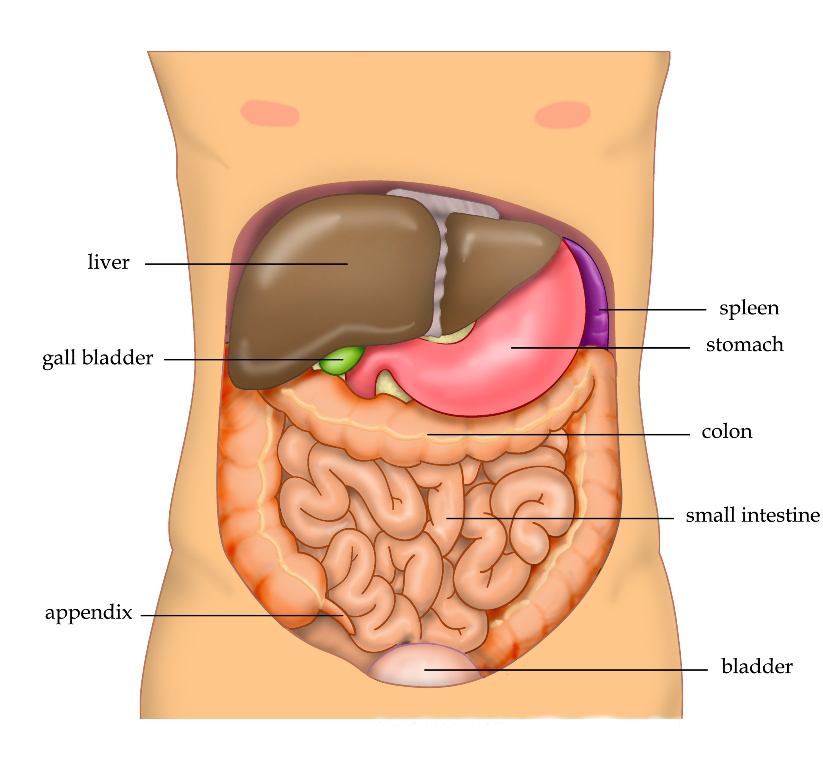
\includegraphics[width = 0.75\columnwidth]{./Images/Chapter1/liverIllustration.jpg}%
\caption{The human liver.}
\label{fig:Ch1LiverAnatomy}
\end{figure}    

Liver cancer is a significant health concern in the United States. Liver cancer can be subdivided into primary liver cancer, where the disease originates in the cells of the liver, and secondary liver cancer, where the cancer originates in other organs and metastasizes to the liver. Approximately 35,660 new cases of primary liver cancer will be diagnosed in the United States in 2015, and approximately 24,550 people will die of these cancers~\cite{AmericanCancer2015}. Secondary liver cancers occur more frequently. Common types of cancer such as breast, lung, and colon all metastasize to the liver. For example, a quarter of the approximately 130,000 patients diagnosed with colorectal cancer each year in the United States will develop liver metastases~\cite{Ananthakrishnan2006,CDC2015,Haddad2011}. Liver cancer is an even more significant health concern in other parts of the world. Liver cancer is the most common type of cancer in many countries in sub-Saharan Africa and Southeast Asia. More than 700,000 people are diagnosed with this cancer each year throughout the world, with more than 600,000 deaths annually~\cite{AmericanCancer2015}.

\subsection{Treatment of Liver Tumors}
Surgery, either for resection of the tumor or a liver transplant, is the only curative treatment of liver cancer, and offers the best long-term survival in select patients. However, approximately three quarters of patients are ineligible for surgery due to tumor size, type, or location; inadequate liver reserve; or other comorbidities. Percutaneous radiofrequency ablation (RFA) is a common, less invasive treatment option for liver cancer patients who are not eligible for resection or transplantation. In this procedure, long electrodes are inserted through the skin into the liver, and are used to ablate the cancer by depositing a high-frequency alternating current into the tissue. 

Current percutaneous RFA of liver cancer suffers from significant limitations~\cite{Gervais2009}. Straight electrodes are unable to reach tumors in some portions of the liver because they are blocked by vasculature, lung, or other sensitive structures. Large tumors require multiple electrode insertions, with each puncture through the liver capsule increasing the risk of hemorrhage. This increased risk can make patients with advanced liver disease or severe comorbidities ineligible for the RFA procedure. Successful treatment requires a margin of cancer-free tissue to be ablated around the tumor, in order to reduce the likelihood of recurrence~\cite{Kim2006}. For medium to large tumors, developing a sufficient ablative margin is highly dependent on the clinician's ability to locate the electrode tip over multiple passes using medical imaging for guidance~\cite{Dodd2001}. 

\subsection{Robotic Needle Steering}
Robotic needle steering enables the insertion of flexible needles along controlled, curved, three-dimensional (3D) paths through tissue~\cite{DiMaio2005,Webster2006}. Robotic needle steering offers the potential to improve percutaneous RFA of liver tumors in several ways. Specifically, robotic needle steering may allow clinicians to (1) correct for errors during insertion and reach a target position with superior accuracy compared to manual insertion, (2) steer around obstacles to previously unreachable targets, and (3) reach multiple targets from a single insertion site, thus reducing the risk of complications such as hemorrhage or infection.

%%%%%%%%%%%%%%%%%%%%%%%%%%%%%%%%%%%%%%%%%%%%%%%%%%%%%%%%%%%%%%%%%%%%%%%%%%%%%%%%%%%%%%%%%%%%%%%%%%%%======================================================================
\section{Prior Work}
%======================================================================
%%%%%%%%%%%%%%%%%%%%%%%%%%%%%%%%%%%%%%%%%%%%%%%%%%%%%%%%%%%%%%%%%%%%%%%%%%%%%%%%%%%%%%%%%%%%%%%%%%%

\subsection{Techniques for Needle Steering}
A number of methods have been described for steering needles through tissue. A recent review is given in~\cite{vandeBerg2014}. DiMaio and Salcudean~\cite{DiMaio2005} and Glozman and Shoham~\cite{Glozman2007} used lateral robotic manipulation of the needle base during insertion to steer the needle. Mallapragada et al.~\cite{Mallapragada2009} and Torabi et al.~\cite{Torabi2009} used robotic manipulation of simulated tissues around a needle during insertion to steer the needle. Okazawa et al.~\cite{Okazawa2005} used a precurved stylet that could be rotated and translated relative to a straight needle shaft to steer a manually inserted needle device. The same concept of overlapping pre-curved sections has been applied in multiple stages in the active cannula robots described by Sears and Dupont~\cite{Sears2006} and Webster et al.~\cite{Webster2009}. Kratchman et al.~\cite{Kratchman2011} described tendon actuation systems designed to steer flexible needle shafts in solid tissue. Ayvali et al.~\cite{Ayvali2012}, Datla et al.~\cite{Datla2014}, and Ryu et al.~\cite{Ryu2014} have described using shape memory alloy (SMA) actuators to articulate needle sections, with the latter system using optically actuated SMA tendons to allow compatibility with MRI systems. Ko and Rodriguez y Baena~\cite{Ko2013} have described a biologically inspired needle that steers by adjusting the relative offset between parallel sections. Our work focuses on bent-tip steerable needles: flexible needle shafts with bent distal sections. These needles naturally steer along curved paths during insertion as a result of the net lateral force acting at the distal end of the needles~\cite{Webster2006}. A duty-cycle control approach, first proposed by Minhas et al.~\cite{Minhas2007}, allows curvature to be varied by alternating periods of needle rotation. A bent-tip needle with a passive flexure was introduced by Swaney et al.~\cite{Swaney2013} to reduce tissue damage caused by the bent tip during rotation. Similar flexible needles with bevel tips~\cite{OLeary2003,Alterovitz2005} and curved distal sections~\cite{Wedlick2009} have also been described. A tendon-actuated bent-tip steerable needle was described by van de Berg et al.~\cite{vandeBerg2015}. This design incorporates a two degree-of-freedom ball and socket joint with a conical tip to achieve 3D steering.

\subsection{Automatic Segmentation of Needles from Ultrasound}
A large amount of prior art exists on the automatic segmentation of needles from B-mode (grayscale) ultrasound data, with much of it focused on segmenting straight needles using a variant of the Hough transform. Although the Hough transform is computationally intensive, real-time segmentation of straight needles has been demonstrated using variations on the algorithm, including dual-plane projections~\cite{Ding2003b}, coarse-fine sampling~\cite{Ding2003a,Zhou2008}, and parallel implementation on a graphics processing unit~\cite{Novotny2007}. Other similar algorithms, such as the parallel integral projection transform, have also been applied~\cite{Barva2008}. Similar methods have been described for segmenting curved needles. Slightly curved needles can be segmented using a standard Hough transform method~\cite{Okazawa2006,Aboofazeli2009}, while more strongly curved needles can be segmented by including a parametrization of needle bending~\cite{Neshat2008,Okazawa2006,Uhercik2010}.

The underlying issue that makes automatic needle segmentation a difficult problem is the poor visibility of needles in standard B-mode ultrasound data. Several of the described methods have shown promising results in favorable conditions. However, image-guided robotic needle steering requires segmentation algorithms that can process large 3D datasets containing highly curved, extremely thin (e.g., 0.5-mm diameter) needles at undesirable orientations relative to the transducer. Rather than contribute a new algorithm that attempts to overcome these challenges, our aim in this work was to reduce the complexity of the segmentation task, by leveraging the needle steering robot to produce ultrasound image data that more clearly reveal the needle.

\subsection{Doppler-Based Segmentation}
Ultrasound Doppler is a diagnostic technique that measures frequency shifts in reflected ultrasonic waves that result from motion. Color and power Doppler imaging, which are available on most modern ultrasound systems, are commonly applied to overlay blood flow data on B-mode ultrasound. Vibrating solid objects have also been shown to produce recognizable Doppler signals~\cite{Holen1985}. This concept has been applied to localize straight needles~\cite{Armstrong2001,Feld1997,Hamper1991} and needle tips~\cite{Harmat2006} in 2D ultrasound, as well as instruments in cardiac interventions~\cite{Fronheiser2008,Reddy2008} and other applications~\cite{McAleavey2003,Rogers2009}. This technique has not previously been applied to segment highly curved needles.

\subsection{Control Approaches for Robotic Needle Steering}
There is significant prior art relevant to image-guided control of needle steering, both for bent-tip steerable needles and other approaches. DiMaio and Salcudean formulated rigid needle insertion as a trajectory planning and control problem, defining a needle manipulation Jacobian for base control~\cite{DiMaio2005}. Glozman and Shoham~\cite{Glozman2007} and Neubach and Shoham~\cite{Neubach2010} used inverse kinematics to control base-manipulation needle steering, with X-ray and ultrasound image feedback respectively. Ko and Rodriguez y Baena used a model-predictive control algorithm for trajectory-following control of a bio-inspired actuated flexible needle~\cite{Ko2012}. For bent-tip steering, a number of control approaches have been described based on a nonholonomic model of steerable needle motion in tissue~\cite{Webster2006}. Reed et al. demonstrated image-guided needle steering in a planar workspace~\cite{Reed2011}, by combining a planar motion planner~\cite{Alterovitz2008}, an image-guided controller~\cite{Kallem2009}, and a torsion compensator~\cite{Reed2009}. Wood et al. formulated trajectory tracking controllers based on duty cycling for 2D~\cite{Wood2010} and 3D~\cite{Wood2013} trajectories. Bernardes et al. combined closed-loop image feedback with intraoperative replanning to deal with obstacles and dynamic workspaces~\cite{Bernardes2013}. Rucker et al.~\cite{Rucker2013} used a sliding mode controller with feedback from an electromagnetic tracking system. This control scheme has the advantage that it does not require any prior knowledge of needle curvature. Abayazid et al. demonstrated bent-tip needle control in gelatin and chicken breast using a robotically controlled ultrasound transducer to track the tip~\cite{Abayazid2014}. The steerable needle described by van de Berg et al.~\cite{vandeBerg2015} uses an integrated fiber Bragg grating (FBG) shape sensor and proportional-integral control of the tendon-actuated tip. 

Several schemes for teleoperation or human-in-the-loop control of steerable needles have been proposed. Romano et al. implemented several joint-space control schemes, comparing autonomous, manual, and combined control of the insertion and rotation of the steerable needle~\cite{Romano2007}. Majewicz and Okamura implemented task-space teleoperation using a 3D display and a haptic device as a master input~\cite{Majewicz2013}. In a human user study, they found task-space teleoperation resulted in lower time to target and insertion length than joint-space teleoperation. Pacchierotti et al. implemented a teleoperation system that combined kinesthetic and
vibratory feedback to provide information about ideal insertion and rotation of the steerable needle~\cite{Pacchierotti2014}.

\subsection{Current State of Needle Steering Research}
Robotic needle steering has existed solely as a research concept for over a decade. The work on rigid needle steering by DiMaio and Salcudean in 2005~\cite{DiMaio2005} appears to be the first in this area. At roughly the same time, Webster et al. suggested using flexible needles with asymmetric tips to steer through solid organs~\cite{Webster2005}. Since then there have been dozens of journal and conference articles on this topic, all motivated by the potential benefits of achieving controlled, curved needle paths through tissue. Interestingly for a medical robotics topic, there has been almost no progression towards clinical or patient studies. Steerable needles have only been applied in one \textit{in vivo} test~\cite{Majewicz2012}, which measured open-loop steerable needle curvature in different tissues, without simulating any clinical scenario or performing any closed-loop targeting.

To date, needle steering research has been largely the domain of roboticists. Experimental validation of many of the methods described above have been limited to artificial tissues. These artificial tissues provide only limited validation, as their mechanical properties are significantly different from biological tissues~\cite{Wedlick2012}. Without methods for medical image feedback, many needle steering experiments have been constrained to 2D workspaces in transparent artificial tissues such as agar or PVC rubber, with optical cameras used to simulate medical imaging. Although some studies have applied more realistic medical imaging methods~\cite{Glozman2007,Neubach2010,Abayazid2014}, they have generally been evaluated in tightly controlled bench-top settings, yielding best-case needle visibility.

The high-level goal of this thesis was to move robotic needle steering closer to the clinical domain, by targeting a specific percutaneous intervention (ablation of liver tumors), and solving several of the largest technical problems specific to that procedure. In particular, we focused on implementing real-time medical image feedback, achieving sufficient curvature in liver tissue, and allowing human-in-the-loop control. In all these areas, our focus was on clinically realistic implementations that were validated in biological tissues.  

%%%%%%%%%%%%%%%%%%%%%%%%%%%%%%%%%%%%%%%%%%%%%%%%%%%%%%%%%%%%%%%%%%%%%%%%%%%%%%%%%%%%%%%%%%%%%%%%%%%%======================================================================
\section{Contributions}
%======================================================================
%%%%%%%%%%%%%%%%%%%%%%%%%%%%%%%%%%%%%%%%%%%%%%%%%%%%%%%%%%%%%%%%%%%%%%%%%%%%%%%%%%%%%%%%%%%%%%%%%%%
The major contributions of the research described in this dissertation can be summarized as follows:
\begin{itemize}
\item Proposed and validated a method for automatic segmentation of a steerable needle from 3D ultrasound data, based on applying mechanical vibration to the steerable needle in order to make it visible in power Doppler ultrasound.
\item Completed a workspace analysis of percutaneous RFA of liver tumors, using medical image analysis to set a procedure-specific requirement for steerable needle curvature.  
\item Performed finite-element modeling and experimental studies to demonstrate that the required steerable needle curvature can be achieved in liver tissue through optimization of tip geometry. Motivated by these results, proposed and validated an articulated-tip steerable needle mechanism.   
\item Implemented and validated a system for freehand-3D-ultrasound-guided needle steering, which allows a clinician to manually visualize target anatomy while simultaneously providing image feedback for automatic control. Proposed and validated an estimation scheme based on an unscented Kalman filter. 
\end{itemize}

%%%%%%%%%%%%%%%%%%%%%%%%%%%%%%%%%%%%%%%%%%%%%%%%%%%%%%%%%%%%%%%%%%%%%%%%%%%%%%%%%%%%%%%%%%%%%%%%%%%%======================================================================
\section{Dissertation Overview}
%======================================================================
%%%%%%%%%%%%%%%%%%%%%%%%%%%%%%%%%%%%%%%%%%%%%%%%%%%%%%%%%%%%%%%%%%%%%%%%%%%%%%%%%%%%%%%%%%%%%%%%%%%
This dissertation is composed of six chapters. This introductory chapter has provided the clinical motivation for the work, a survey of relevant research literature, and a summary of the contributions of the dissertation. Chapter 2 describes methods for automatic segmentation of a steerable needle from 3D ultrasound data. Chapter 3 describes the workspace analysis of percutaneous RFA of liver tumors, as well as finite-element modeling, experimental studies and mechanism design intended to achieve improved steerable needle curvature in liver tissue. Chapter 4 describes a new estimation scheme based on an unscented Kalman filter, which is used to improve closed-loop steering results with noisy ultrasound measurements.
Chapter 5 combines elements from the previous chapters, in order to demonstrate human-in-the-loop control of ultrasound-guided needle steering. Finally, Chapter 6 summarizes the results of the research, reviews the contributions made in this dissertation, and provides suggestions for future work.